% Add \usepackage{graphicx} to the manuscript preamble if needed.
% Copy the two PDFs next to the manuscript, or adjust the paths below.
% figure* uses the full text width in a two-column journal layout.
% This is a standalone insertion fragment; the manuscript is not modified.

\begin{figure*}[t]
  \centering
  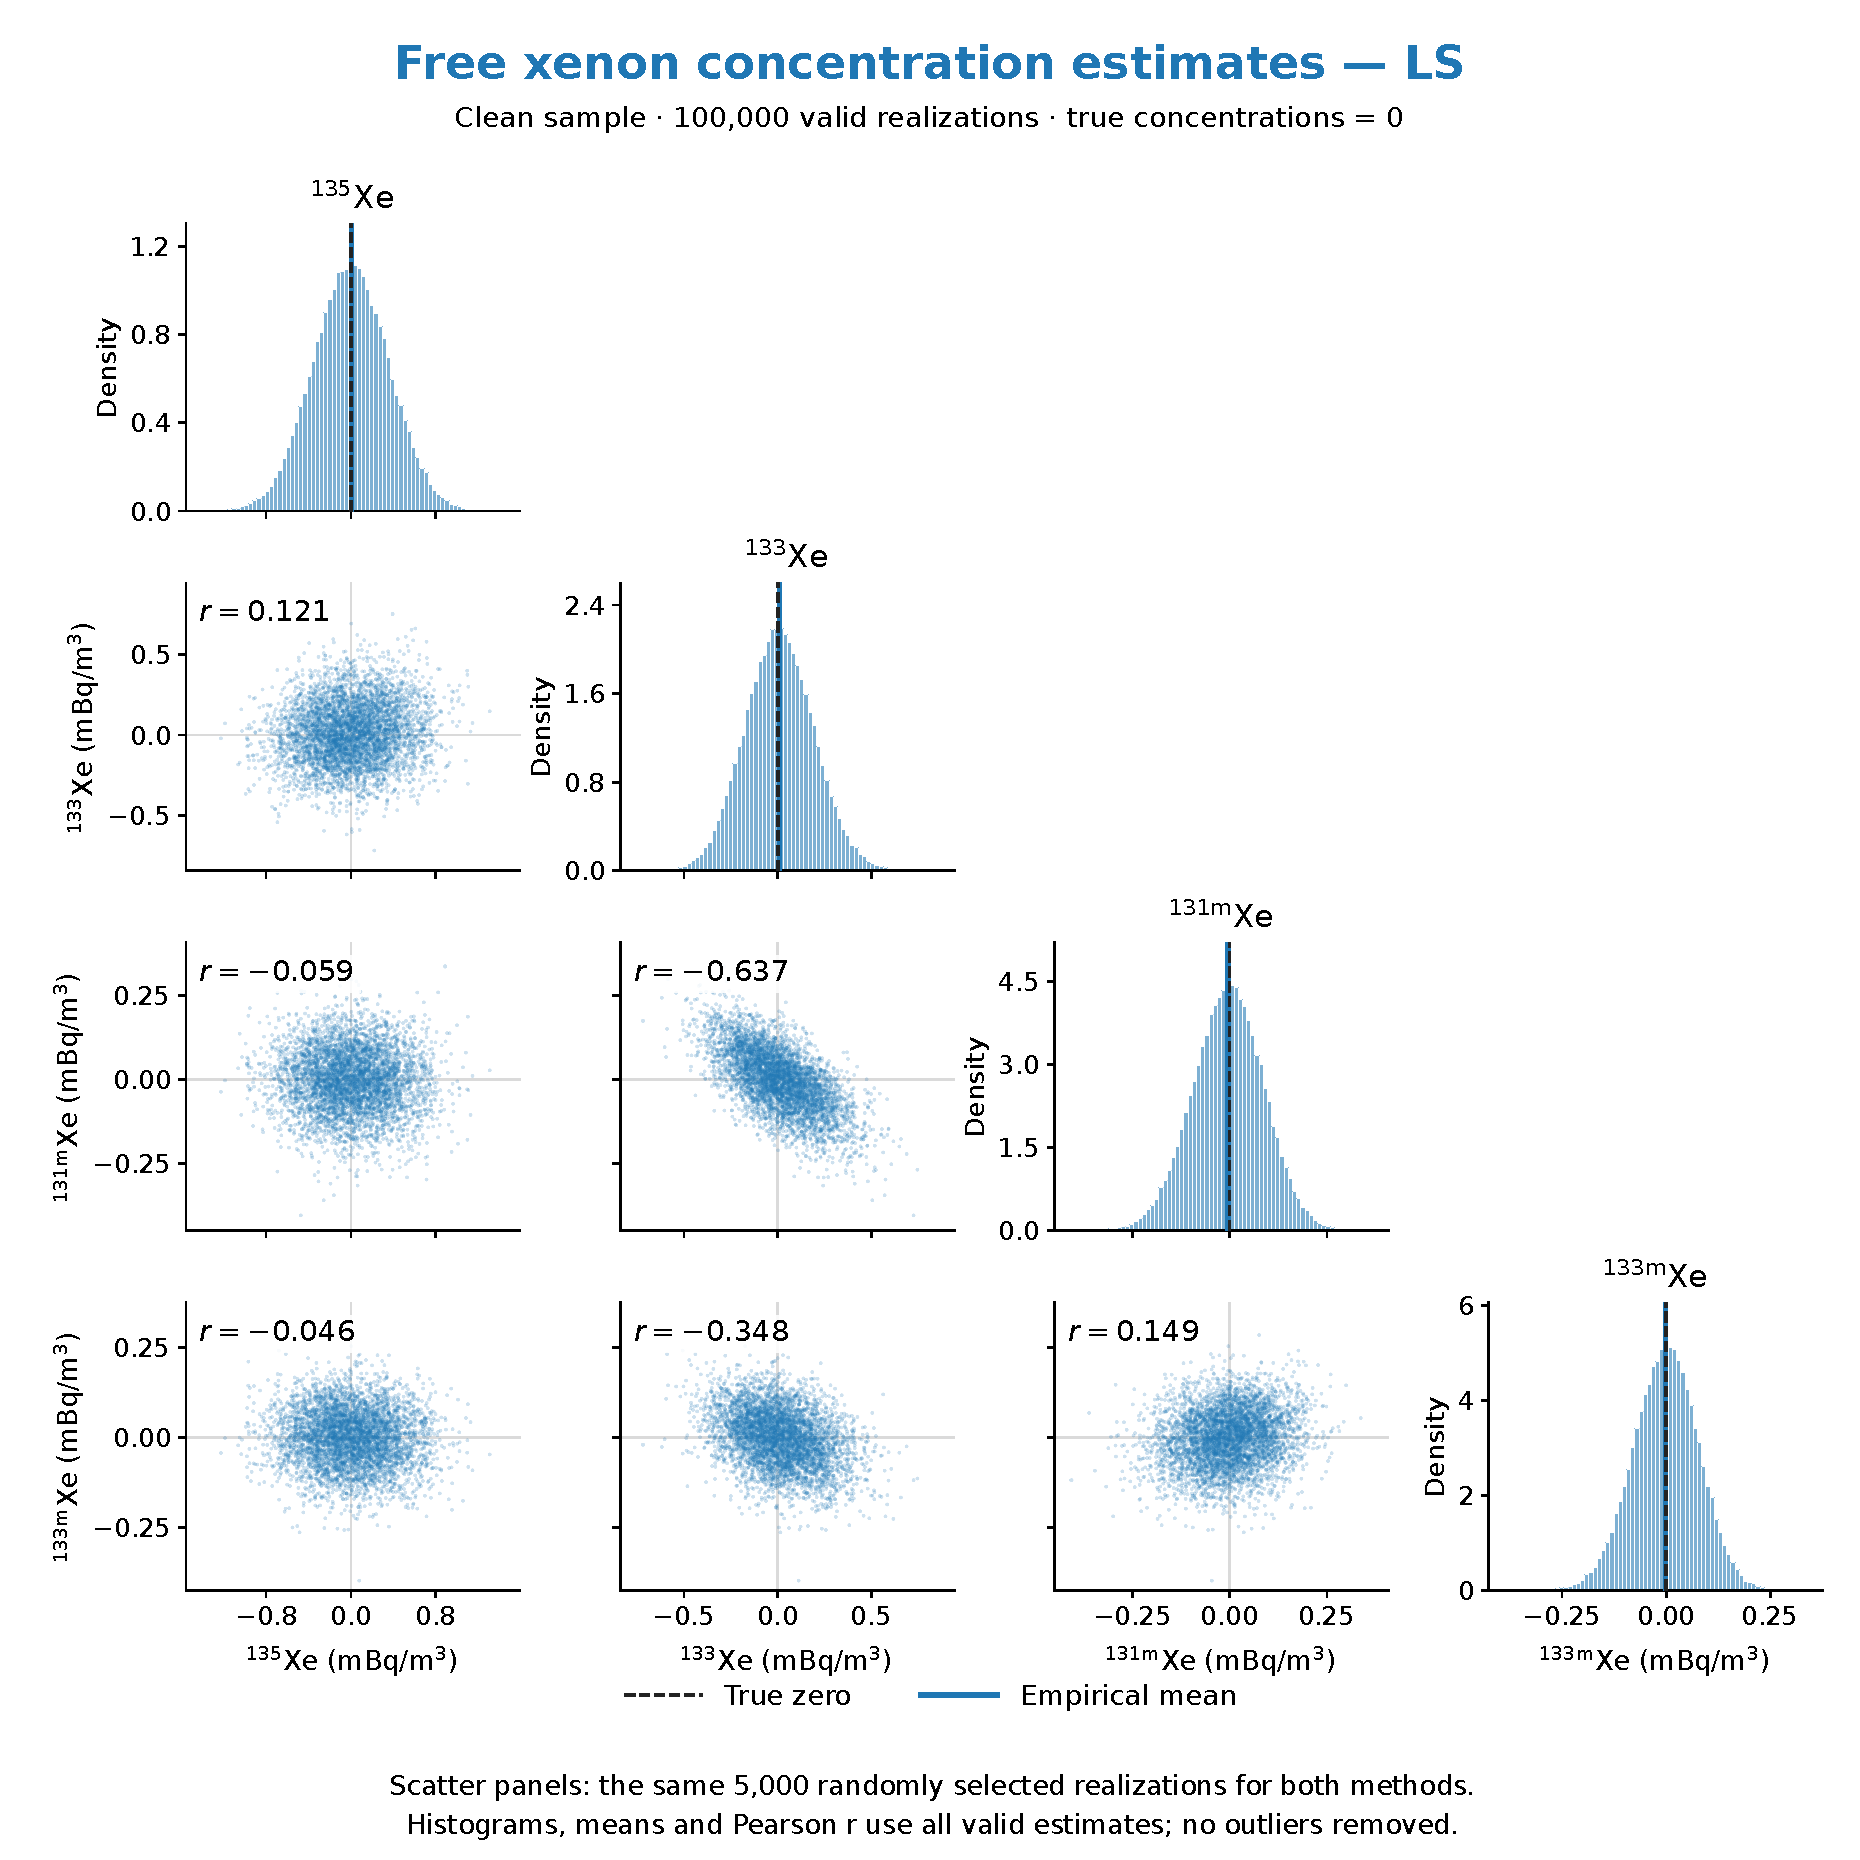
\includegraphics[width=\textwidth]{corner_ls.pdf}
  \caption{Free xenon concentration estimates from weighted least squares (LS)
  for a clean sample with detector background. True fresh-sample and memory
  activities, including radon, are zero. Histograms and Pearson correlations
  use all 100\,000 realizations; scatter panels use 5\,000 shared indices.
  Vertical lines mark zero and the empirical mean. Concentrations are in
  $\mathrm{mBq}\,\mathrm{m}^{-3}$; axes and bins match
  Fig.~\ref{fig:xemat-clean-poisson}.}
  \label{fig:xemat-clean-ls}
\end{figure*}

\begin{figure*}[t]
  \centering
  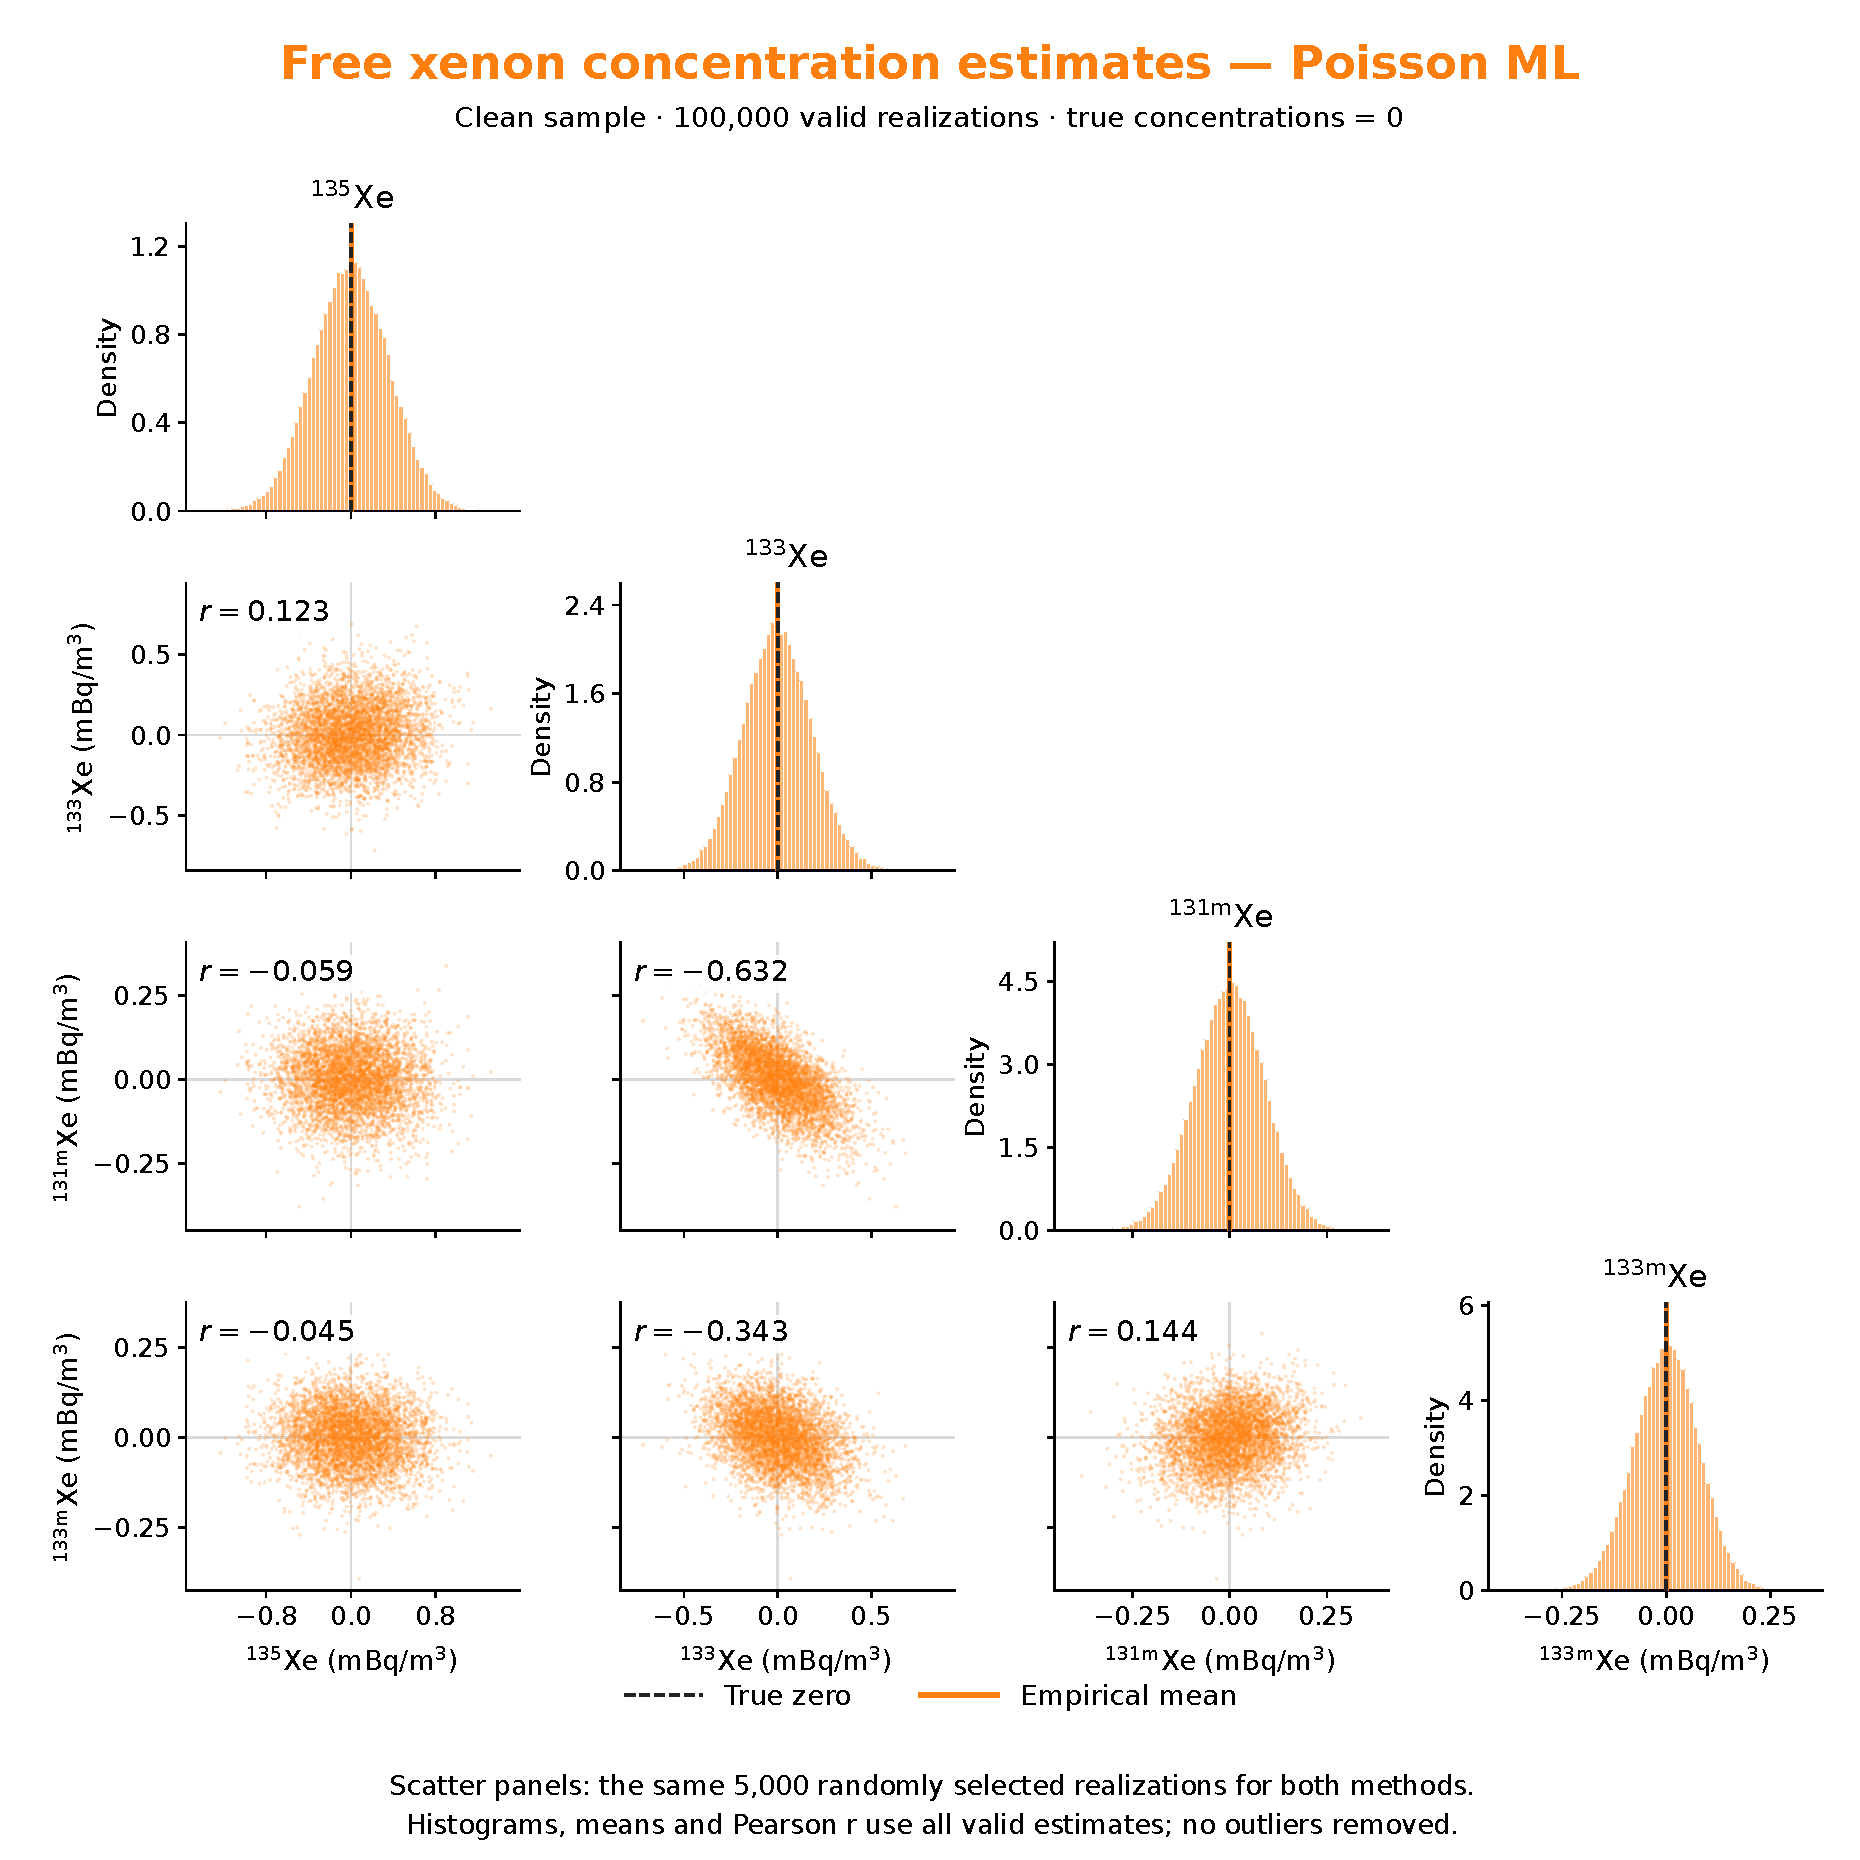
\includegraphics[width=\textwidth]{corner_poisson_ml.pdf}
  \caption{Free Poisson maximum-likelihood (ML) estimates from the same
  100\,000 Poisson-generated SAMPLE, GASBK and DETBK observation vectors as
  in Fig.~\ref{fig:xemat-clean-ls}. Histograms and Pearson correlations use
  all realizations; scatter panels use the same 5\,000 indices as LS.
  Vertical lines mark zero and the empirical mean. Concentrations are in
  $\mathrm{mBq}\,\mathrm{m}^{-3}$. Negative estimates and outliers are retained.}
  \label{fig:xemat-clean-poisson}
\end{figure*}
